\sloppy
\documentclass[14pt,a4paper,oneside]{extarticle}	% Размер основного шрифта и формата листа
\usepackage{xltxtra}						% Используется для вывода логотипа XeLaTeX
\usepackage{xunicode}						% Кодировка документа
\usepackage{polyglossia}					% Загружает пакет многоязыковой верстки
\newfontfamily\russianfont{Book Antiqua}
%\setmainfont{Liberation Serif}						% Основной шрифт текста
\setmainfont{Book Antiqua}
\setdefaultlanguage{russian}				% Основной язык текста
\setotherlanguage{english}					% Дополнительный язык текста
\linespread{1}							% Межстрочный интервал выбран полуторным
\usepackage[left=2.5cm,
right=1.5cm,vmargin=2.5cm]{geometry} % Отступы по краям листа
\bibliographystyle{ugost2008}

\usepackage{xcolor}
\usepackage{hyperref}
% Цвета для гиперссылок
\definecolor{linkcolor}{HTML}{359B08} % цвет ссылок
\definecolor{urlcolor}{HTML}{799B03} % цвет гиперссылок
\hypersetup{pdfstartview=FitH,  linkcolor=linkcolor,urlcolor=urlcolor, colorlinks=true}

%---------------------------%
%---- Пакеты расширений ----%
%---------------------------%
\usepackage{xcolor}
\usepackage{hyperref}
% Цвета для гиперссылок
\definecolor{linkcolor}{HTML}{359B08} % цвет ссылок
\definecolor{urlcolor}{HTML}{799B03} % цвет гиперссылок
\hypersetup{pdfstartview=FitH,  linkcolor=linkcolor,urlcolor=urlcolor, colorlinks=true}


\usepackage{verbatim,indentfirst}
\usepackage{cite,enumerate,float}
\usepackage{amsmath,amssymb,amsthm,amsfonts}

%---------------------------%
%--- Вставка иллюстраций ---%
%---------------------------%
\usepackage{graphicx}
\usepackage{subfigure}
%\graphicspath{{Images/}}
\usepackage{fontspec}

\begin{document}
%	\pagestyle{empty} %  выключаенм нумерацию
%\setcounter{page}{3}% Нумерация начинается с третьей страницы
%\renewcommand{\contentsname}{\center{Содержание}}
%\tableofcontents
	
	\begin{center}
		%\addcontentsline{toc}{section}{Опыт 16. Нахождение центра масс}
		\subsection*{Отвесы на вращающейся платформе}
	\end{center}
	
	\begin{figure}[H] 	
		\centering 	
		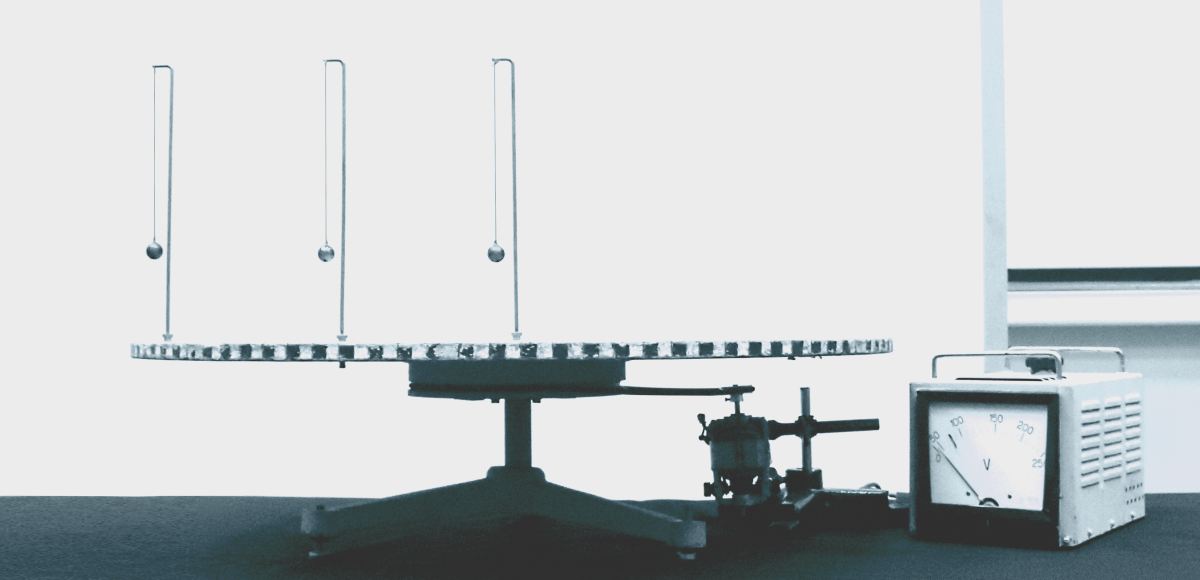
\includegraphics[width=0.9\linewidth]{platform-1.png}
		\caption{Демонстрация центробежной силы инерции}
		\label{platform-1}
	\end{figure}
	
	\subsection*{\underline{Оборудование:}}

	\begin{enumerate} 
		\item Шарики одинакового размера и массы, подвешенные на специальных стойках
		\item Платформа с отверстиями для закрепления стоек с шариками
		\item Электродвигатель с фрикционным индуктором
		\item Вращающаяся подставка для платформы
		\item Резиновое кольцо для передачи вращательного момента от вала двигателя к платформе
		\item Лабораторный трансформатор (ЛАТР)
	\end{enumerate}

	\newpage
	\subsection*{\underline{Основные определения:}}
		
		Центробежная сила инерции — сила, действующая на материальную точку, 
		направленная по главной нормали к ее траектории в сторону центра кривизны 
		(к центру окружности при движении точки по окружности).
		Численно центробежная сила равна $ mv^2/l $, где \textit{m} — масса точки, \textit{v} — модуль ее линейной скорости, \textit{l} — радиус кривизны траектории.
		Под действием центробежной силы материальная точка движется криволинейно. 
		Поэтому при прямолинейном движении эта сила равна нулю.
		
		Нормальное ускорение является составляющей полного ускорения точки при криволинейном движении.
		Направлено такое ускорение по главной нормали к траектории в сторону центра кривизны.
		Обычно термин «нормальное ускорение» применяют в случае движения точки по окружности.
		
		Численно нормальная составляющая ускорения материальной точки равна $ v^2/l $, где \textit{v} — скорость точки, \textit{l} — радиус кривизны траектории.
		При движении по окружности нормальное ускорение может вычисляться по формуле $$ a = R\omega^2, $$ где \textit{R} — радиус окружности, $ \omega $ — угловая скорость вращения этого радиуса. 
		В случае прямолинейного движения нормальное ускорение также как и центробежная сила инерции обращается в нуль.

	\newpage
\subsection*{\underline{Краткое описание:}}
			
		На вращающейся подставке укрепляют деревянный диск, вдоль радиуса которого на равных расстояниях друг от друга располагаются отвесы с металлическими шариками (рис.\ref{platform-2}).
		Первый отвес находится на оси вращения диска, поэтому на него при вращении диска не действует центробежная сила инерции и шарик не отклоняется.
					\begin{figure}[H] 
			\centering 		
			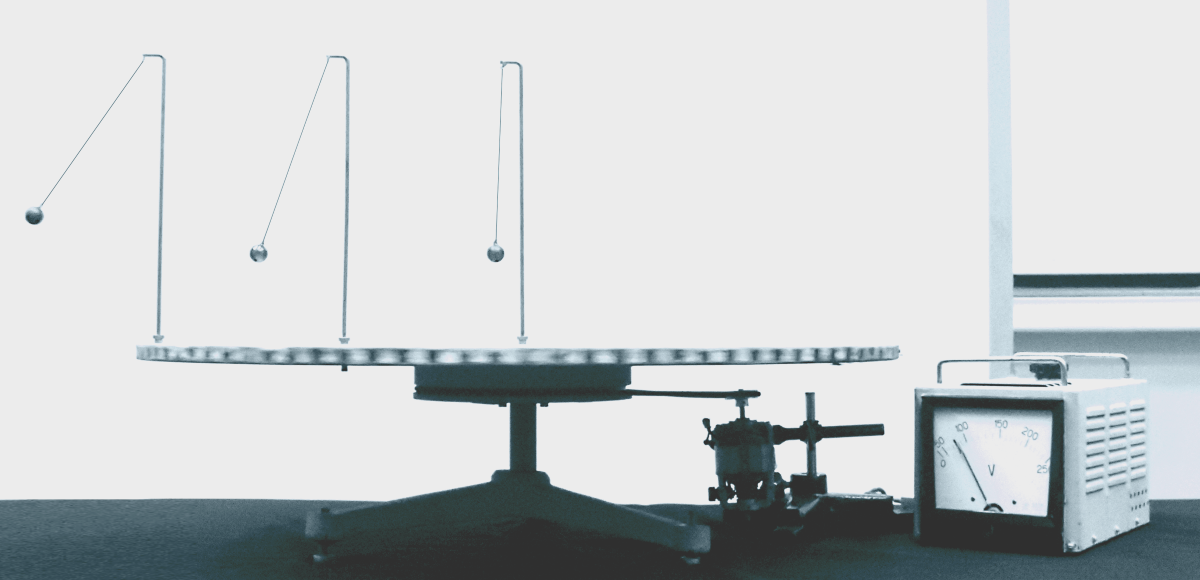
\includegraphics[width=0.9\linewidth]{platform-2.png} 
			\caption{Отклонение маятников от вертикали на вращающейся платформе. В зависимости от расстояния до оси вращения на одинаковые тела будут действовать различные силы инерции. О величине этих сил можно косвенно судить по величине угла отклонения каждого отвеса}
			\label{platform-2}
		\end{figure}
	
		На остальные отвесы действует центробежная сила инерции, пропорциональная расстоянию от оси вращения соответствующего отвеса.
		Поэтому все шарики отклоняются на различные углы, тем больше, чем больше их расстояние от оси вращения.

\newpage
\subsection*{\underline{Теория:}}

При вращении платформы с постоянной угловой скоростью $ \omega $ отвесы маятников отклоняются от вертикального положения, причем углы отклонения отвесов будут тем большие, чем дальше от центра платформы располагаются отвесы (рис.\ref{platform-3}).

Рассмотрим отклонения отвесов маятников относительно наблюдателя, находящегося в инерциальной
системе отсчета \textit{XY} (связана с Землей), и относительно наблюдателя, находящегося в неинерциальной вращающейся системе \textit{xy} (связана с вращающейся платформой). 

\begin{figure}[H] 
	\centering 		
	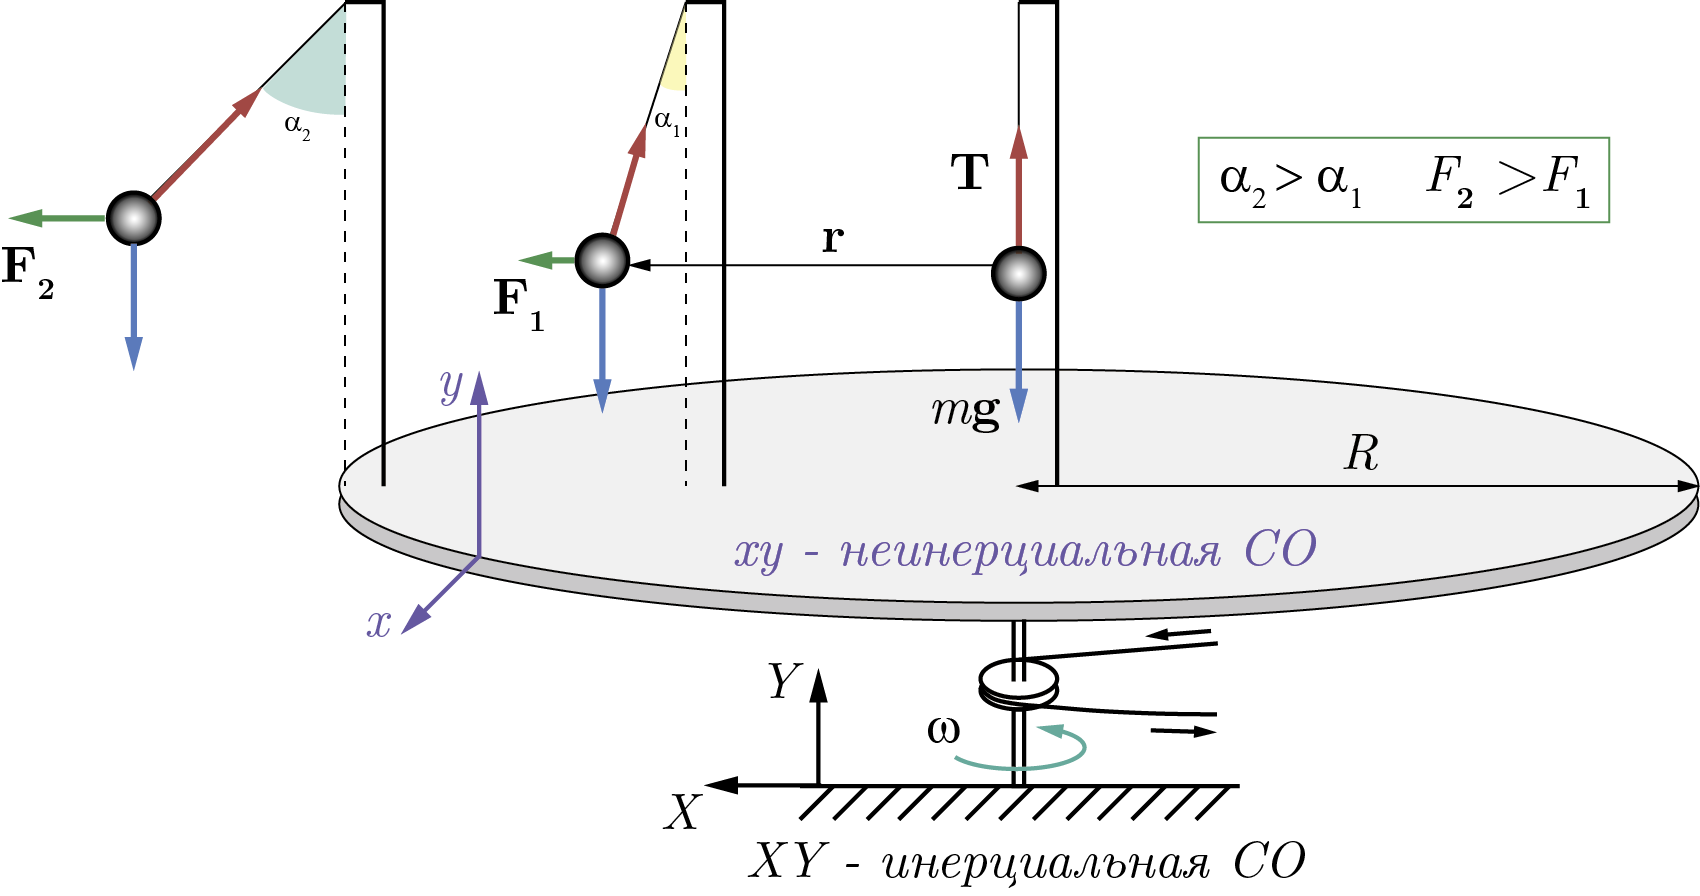
\includegraphics[width=0.9\linewidth]{platform-3.png} 
	\caption{Схематичное изображение поведения грузов на вращающейся платформе, расстояние от каждого из которых до оси вращения различается}
	\label{platform-3}
\end{figure}

Относительно наблюдателя в ИСО отвесы отклоняются, а груз в этом случае находится под действием двух реальных сил: силы тяжести $ m\textbf{g} $ и силы натяжения нити $ \textbf{T} $.
Результирующая сила сообщает маятнику нормальное ускорение $ \textbf{a}_{\text{н}} = -\omega^{2}\textbf{r}  $, поэтому можно записать

\begin{equation}\label{platform-1eq1}
m\textbf{g}+\textbf{T}=-m\omega^{2}\textbf{r},
\end{equation}
где $ \textbf{r} $ — радиус-вектор, проведенный от оси вращения платформы до рассматриваемого груза.

Угол отклонения отвесов будет определяться соотношением:

\begin{equation}\label{platform-1eq2}
\text{tg} \alpha =\frac{m\omega^{2}r}{mg} = \frac{\omega^{2}r}{g}.
\end{equation}

Относительно наблюдателя, находящегося в НИСО (на подвижной платформе), при равномерной скорости вращения отвесы остаются в покое (неподвижны относительно наблюдателя).
Из этого следует, что сумма всех сил, действующих на груз $ m $, в этой системе отсчета должна обращаться в нуль.
Таким образом, наблюдатель, вращающийся вместе с грузами в системе отсчета \textit{xy} может сделать вывод, что на каждый маятник должна действовать некоторая сила, уравновешивающая известную пару реальных сил (притяжения и реакции со стороны подвеса).
Причем эта сила будет обязательно направлена из центра вдоль Вектора \textbf{r}. 
В качестве такой силы обычно рассматривается центробежная сила инерции \textbf{F} (рис.\ref{platform-3}), которая по своей природе является силой инерции.

Запишем уравнение движения маятника во вращающейся системе отсчета в векторной форме с учетом этой силы
\begin{equation}\label{platform-1eq3}
m\textbf{g}+\textbf{T}+\textbf{F}=0.
\end{equation}

Сравнивая его с выражением (\ref{platform-1eq1}), видим, что центробежная сила инерции может быть определена как $ \textbf{F}=m\omega^{2}\textbf{r} $.

Величина центробежной силы инерции, действующей на тела во вращающихся системах отсчета, зависит только от угловой скорости вращения $ \omega $ этой системы отсчета и от расстояния \textit{r} до оси вращения.
Важно, что она не зависит от скорости тел относительно вращающихся систем отсчета.
Иными словами, центробежная сила инерции действует во вращающихся системах отсчета на все без исключения материальные тела независимо от того, покоятся ли они в этих системах или движутся с некоторой относительной скоростью.
				
\end{document}